\documentclass[tikz]{standalone}
\usepackage{pgfplots}
\pgfplotsset{compat=1.18}
\definecolor{bgdark}{HTML}{171D2B}
\definecolor{aksen}{HTML}{F7B538}
\begin{document}
\pagecolor{bgdark}
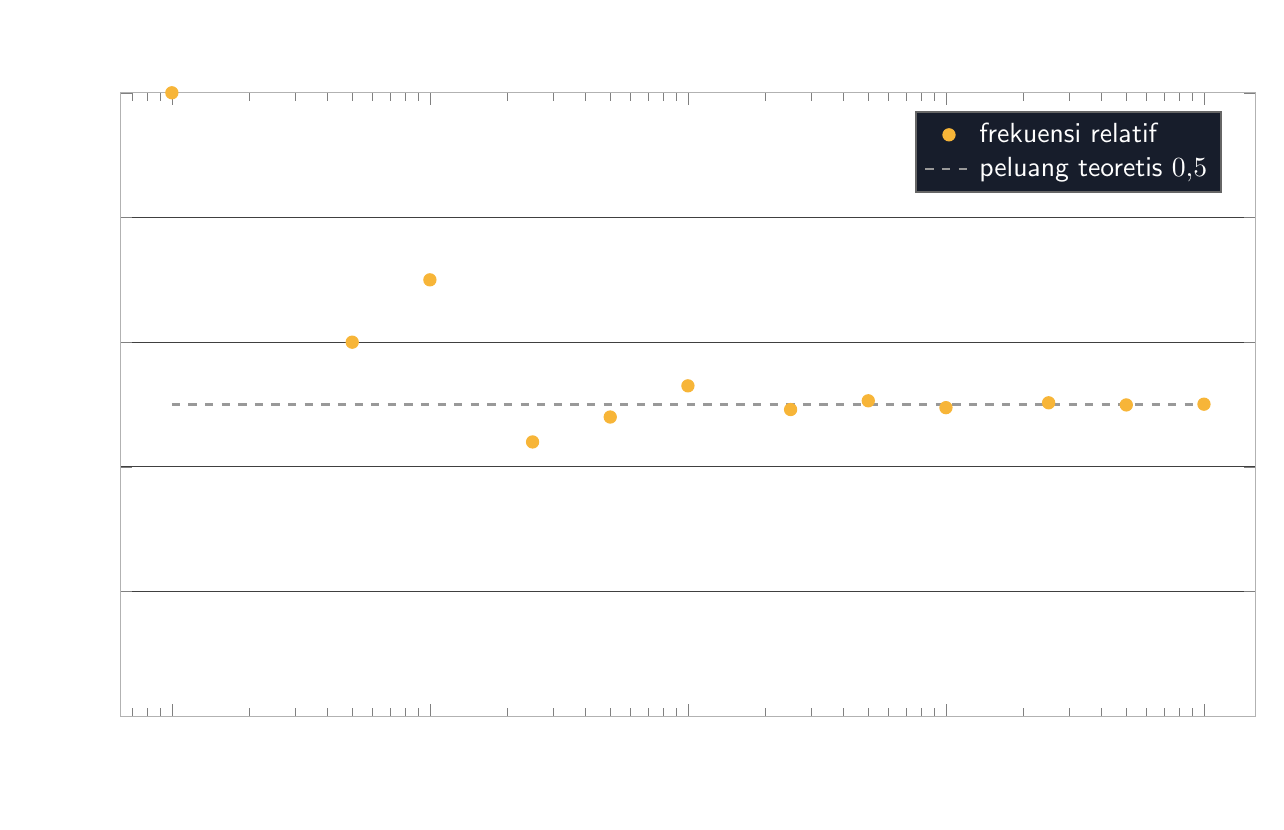
\begin{tikzpicture}[text=white,font=\sffamily]
\begin{axis}[
  width=16cm, height=9.5cm,
  axis line style={white!70!black},
  title={Frekuensi Relatif Angka pada Lemparan Koin},
  title style={font=\bfseries\large},
  xlabel={Banyak lemparan $n$}, ylabel={Frekuensi relatif},
  ymin=0, ymax=1,
  xmode=log, log basis x=10,
  xmin=1, xmax=10000,
  enlarge x limits=0.05,
  ymajorgrids=true, grid style={white!25!black},
  legend pos=north east,
  legend style={draw=white!40!black, fill=bgdark},
  legend cell align=left,
]
\addplot[only marks, mark=*, mark size=2.2pt, color=aksen] coordinates
{(1,1) (5,0.6) (10,0.7) (25,0.44) (50,0.48) (100,0.53) (250,0.492) (500,0.506) (1000,0.495) (2500,0.5028) (5000,0.4994) (10000,0.5006)};
\addlegendentry{frekuensi relatif}
\addplot[white!60!black, thick, dashed, domain=1:10000, samples=2] {0.5};
\addlegendentry{peluang teoretis $0{,}5$}
\end{axis}
\end{tikzpicture}
\end{document}
